\section*{Event Reconstruction in CMS}

The reconstruction of a collision event requires the identification of all produced particles in the CMS detector. Particles are identified based on their signature in the sub-detectors sensitive to that particle. This chapter describes the concepts and the most relevant details of the CMS event
reconstruction algorithms and particles identification algorithms. The event reconstruction can be divided into three steps. \\
\begin{wrapfigure}{r}{0.55\textwidth}
    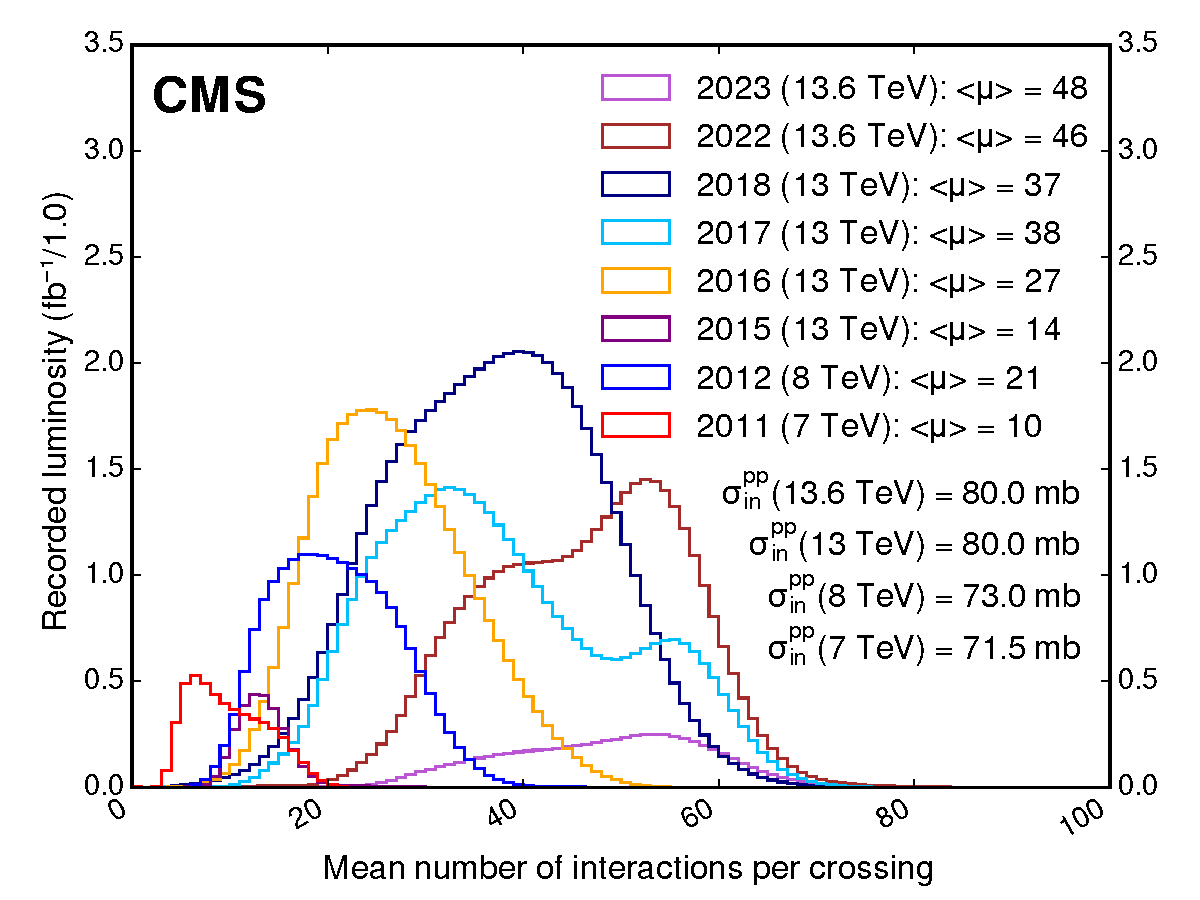
\includegraphics[width=0.55\textwidth]{pileup_allYears.pdf}
    \caption{Interactions per bunch-crossing (pileup) for 2011-2012 and 2015-2018 and 2022-2023}
    \label{Fig:PileUp}
\end{wrapfigure}
The first step in event reconstruction is the reconstruction of particle tracks and event vertices. The collision of protons in the detector can occur a number of times per bunch crossing spread along the beam axis which is called pile-up (PU). Pile-up gives rise to a series of event vertices: the centre of a proton-proton collision in the event from which particles are produced. The primary vertex (PV) is defined as the one with the largest value of summed transverse momentum, other vertices are tagged as pile-up. To reconstruct event vertices particle racks are reconstructed first and are then associated to vertices. particle track reconstruction is based on a combinatorial Kalman filter method\cite{BILLOIR1990219}. This filter works iteratively starting from an estimate of the 
particle track and including information of the successive detection layers one by one to re-estimate the track. The re-estimation of the track uses a refitting by a least-squares approach on each successive hit and tracks that 
do not satisfy goodness-of-fit criteria are discarded. In addition, particle tracks are required to originate from within a few mm in radius around the beam axis and to have a pT larger than 0.9 GeV in order to be counted as this cut reduces fake track identification due to false hits in the detector\cite{Sirunyan_2017}. Easier to reconstruct tracks are reconstructed first, this includes high $p_T$ and close to the interaction point tracks. Hits from reconstructed tracks are then removed simplifying the reconstruction for further iterations of more complex tracks.

Reconstruction of event vertices are based on all reconstructed tracks and are initially estimated by a grouping of the track with similar coordinates along the beam-axis and closest approach to the centre of the beam spot. An adaptive vertex fitter\cite{Fruhwirth:2007hz} is then used to optimise the  assignment of reconstructed tracks to vertices. in an adaptive vertex fitter the probability of a track to originate from a specific vertex is assigned as weight to that track. Vertex weights are derived as the sum of the weights of all associated tracks, and interaction vertices with weights below a certain thresholds are removed. This results in a set of defined pile-up vertices and one primary vertex with respective tracks.\\
\\
\begin{figure}[t]
    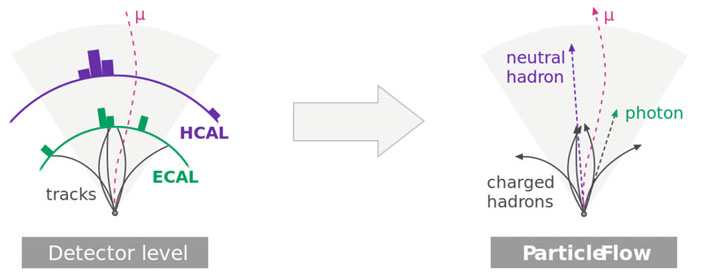
\includegraphics[width=1.0\textwidth]{ParticleFlow.png}
    \caption{The particle-flow algorithm combines information from various subdetectors to provide a global description of the event in terms of electrons, photons, muons, charged hadrons, and neutral hadrons\cite{Defranchis:2020efl}}
    \label{Fig:P}
\end{figure}
A second step is \textbf{Particle-flow reconstruction}. Here the Particle-flow (PF) algorithm aims to combine information of different sub-detectors and track reconstruction to reconstruct and classify PF-candidates: electrons, photons, muons, charged hadrons, or neutral hadrons. The algorithm can be divided in two stages: the reconstruction of the PF elements and the linking of PF-elements to reconstruct a particle. PF-elements are objects constructed from combining sub-detector information and include charged tracks, muon tracks, and calorimeter clusters. Charged tracks are fitted from hits in the tracking system as explained above. Muon tracks are fitted from information of both the muon system and the tracking system. Last, calorimeter clusters are defined by a clustering algorithm that bundles neighbouring deposits in the ECAL or HCAL. The linking of PF-elements first proceeds with a link algorithm that tests any pair of PF-elements for a link based on specific criteria. The link between a charged track and a calorimeter cluster is worked out as example. The track is extrapolated to the ECAL layer and HCAL layer. The track is linked to the cluster if its extrapolated position is within the area of the calorimeter cluster in the ($\eta,\phi$) plane. In the case of multiple ECAL or HCAL clusters linked to one charged path, the closest calorimeter cluster is kept. The end-result of the PF algorithm are particle candidates that can further be used to select electrons, muons, photons and reconstruct jets from charged and neutral hadrons.

The last step in the event reconstruction process is \textbf{jet clustering and tagging}. As discussed quarks and gluons produced in proton collisions are not detectable in the experiment but form a hadron shower to be detected instead. To reconstruct these original quarks and gluons jets are clustered from all PF-candidates. The method to cluster jets uses a sequential clustering algorithm "anti-kT"\cite{Cacciari_2008}. This jet-clustering algorithm uses an iterative process as follows. On each iteration it starts by identifying the smallest distance $d_{ij}$ between objects (a PF-candidate or cluster of sub-jet) or distance $d_{iB}$ between an object and the beam-line $B$ calculated as
\begin{align}
    d_{ij} &= \min(p_{T_i}^{-2},p_{T_j}^{-2}) \frac{\Delta R^2_{ij}}{R^2} \\
    d_{iB} &= p_{T_i}^{-2}
\end{align}
with $\Delta R^2_{ij} = (\phi_i-\phi_j)^2+(\eta_i-\eta_j)$ and $R$ a distance parameter that controls the size of the jet. If the smallest distance is of the form $d_{ij}$ the objects $i$ and $j$ are combined to form a cluster of PF-candidates als known as a sub-jet. If the smallest distance is of the form $d_{iB}$ the object $i$, most often a sub-jet, is tagged as a jet and is removed from the list of objects to cluster. This procedure of clustering is repeated until no entities are left to cluster. \\
\\
The presence of PF-candidates from PU vertices can however influence the jet clustering algorithm and the jet properties obtained from jet clustering. To prevent this, two approaches for PU mitigation in jet clustering exist. A first approach is to start by remove charged PF-candidates that do no originate from the primary vertex prior to jet clustering. Next, to consider the energy of neutral PF-candidates and remaining charged PF-candidates from PU vertices that were not removed a correction is applied to the four-momentum of the jets after clustering. The second approach is pileup per particle identification (PUPPI)\cite{Bertolini_2014} and uses shape information, event pileup properties and tracking information to counteract PU effects before jet clustering. The PUPPI algorithm first selects a shape $\alpha$ that aims to distinguish particles from PU-vertices and particles from the primary vertex and computes it for each PF-candidate in the event. This shape $\alpha$ encapsulates shape information of particle properties that differ between particles of the PU and primary vertex (e.g. the transverse momentum $p_T$ of PF-candidates from PU falls of faster at high $p_T$). To characterise the PU distribution, the algorithm calculates the median and root mean square of the $\alpha$ values for known charged PF-candidates from PU. These values give information into the overall PU distribution. Each PF-candidate is assigned a weight based on a comparison between its $\alpha$ value and the median of the charged PU distribution. The weight ranges from zero to one where PF-candidates from PU are often assigned a weight close to zero and PF-candidates from the primary vertex are preferably assigned a weight close to one. Finally, the PF-candidate weights are applied to rescale their four-momentum and PF-candidates with very small weights are removed. The resulting set of pileup-corrected PF-candidates can be used as input for jet clustering. \\
\begin{wrapfigure}{r}{0.55\textwidth}
    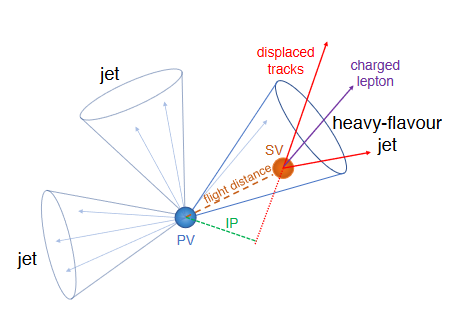
\includegraphics[width=0.55\textwidth]{bjet.png}
    \caption{llustration of a heavy-flavour jet from the decay of a b hadron.\cite{Sirunyan_2018}}
    \label{Fig:Bjet}
\end{wrapfigure}
\\
Jets acquired from the jet clustering algorithm give an estimate of basic properties of the original quark or gluon. A crucial property of the jet still unknown is the hadron; more specifically whether a jet originates from a heavy-flavour hadron. Algorithms exist that identify heavy-flavour jets and use heavy-flavour jet specific properties to distinguish them from light-flavour jets. For example, b-hadrons have a lifetime of the order of 1ps and thus at high enough $p_T$ travel away from the primary vertex before decaying and forming a hadron shower. This shows in the track reconstruction as tracks displaced from the primary vertex. Such a secondary vertex (SV) is thus a signature to help identify b jets, jets originating from b-hadron decay, in jet tagging algorithms. In addition, decay products of heavy-flavour hadrons have on average a higher $p_T$ due to the high b- and c-quark mass. Last, in the decay products of b hadrons around 20\% are charged leptons. These are all discriminating properties that are used in jet tagging algorithms.\\
\\
The combined secondary vertex (\textbf{CSVv2}) algorithm is a jet tagging algorithm that combines the information of displaced tracks with the information on SVs associated with the jet. CSVv2 is based on a fully-connected neural network with binary classification and identifies jets with $p_T$ > 20GeV and at least two reconstructed tracks with $p_T$ > 1GeV by assigning a score that corresponds to the probability of the jet being a b jet. Training of the CSVv2 algorithm is done in three independent categories of jets as the tracks and SV input variables change dependent on the category.
\begin{itemize}
    \item \textbf{RecoVertex}: The jet contains one or more SVs
    \item \textbf{PseudoVertex}: No SV is found in the jet but the jet has least two high-quality tracks\footnote{A high-quality track is defined as a track with a 2D impact parameter significance (the distance between the PV and the track at its points of closest approach divided by its uncertainty) above two and a combined invariant mass of at least 50MeV away from the $K_S^0$.}.
    \item \textbf{NoVertex}: Jets not assigned to the RecoVertex or PseudoVertex categories.
\end{itemize}
One of the important discriminating variables is the track impact parameter (IP), defined as the distance between the PV and the track at its points of closest approach of a track. Tracks from SVs are expected to have an angle between
the jet and the IP lower than $\pi/2$, while the angle between
the jet and the IP of a track from the PV is uniformly distributed. This variable however requires the jet to contain one or more SVs to be used in the CSVv2 algorithm and is thus restricted to the RecoVertex category. An other variable specific to the RecoVertex category is the SV flight distance, defined as the distance between the SV and the PV as shown in Fig. \ref{Fig:Bjet}. A summary of discriminating variables used in the CSVv2 neural network and their applicability in jet categories is given in table 2.1.\\ 
\\
\textbf{DeepCSV}\cite{Sirunyan_2018} is an improved jet tagging algorithm based on the previous CSVv2 tagger. DeepCSV is a multi-classifier machine learning algorithm based on a deep neural network with almost the same input variables as the CSVv2 tagger. Additional input variables of the DeepCSV algorithm are the jet $p_T$ and $\eta$ distributions as well as restricting the number of track-based variables to up to six tracks. Training 
\begin{wrapfigure}{r}{0.6\textwidth}
    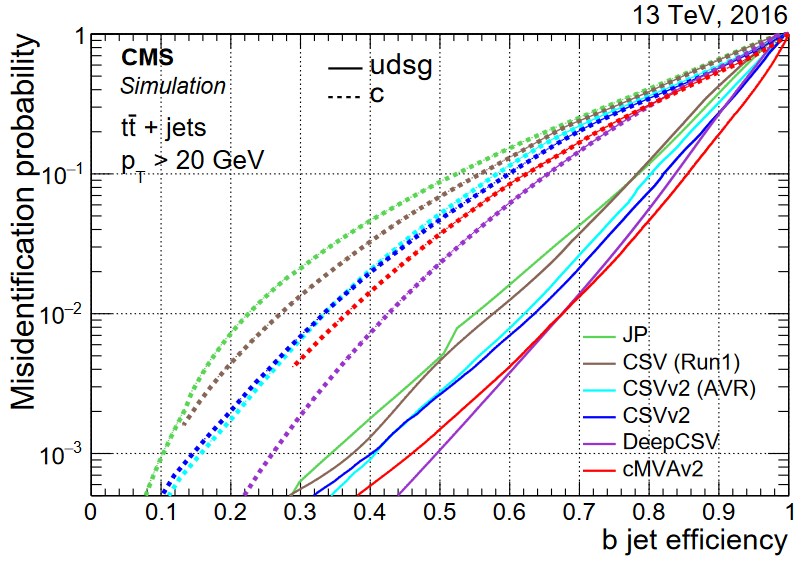
\includegraphics[width=0.6\textwidth]{btaggingEfficiency.png}
    \caption{Misidentification probability of b taggers for light jets (udsg) and c jets in terms of b jet efficiency\cite{Sirunyan_2018}}
    \label{Fig:btagging}
\end{wrapfigure} of DeepCSV happens simultaneous in all jet categories. Discrepancies between categories in the case where a variable can not be reconstructed are solved by setting the value of associated variables to zero. As mentioned, DeepCSV is a multi-classifer and thus can classify a jet into one of the five classes: one b hadron in the jet (b), two b hadrons in the jet (bb), one c hadron in the jet (c), two c hadrons in the jet (cc), or none of the above (udsg), e.g. the jet originates from an up/down/strange quark or gluon. The optimal b tagging efficiency with DeepCSV is achieved by combining the probabilities P(b) and P(bb) of the multi-classifier and use this as binary classification of b tagging. An overview of the b tagging efficiency with generations of jet tagging algorithms applied to jets in top-quark pair simulated events can be seen in Fig. \ref{Fig:btagging}.

\begin{table}[htp]
\begin{tabular}{cccc} 
Input variables & RecoVertex & PseudoVertex & NoVertex\\ 
\midrule
SV 2D flight distance significance & o & x & x\\
Number of SVs & o & x & x\\
Track $\eta_{rel}$ & o & o & x\\
Corrected SV mass & o & o & x\\
Number of tracks from SV & o & o & x\\
SV energy ratio & o & x & x\\
$\Delta R$ (track jet) & o & o & x\\
3D IP significance of the first four tracks & o & o & o\\
Track $p_{T,rel}$ ratio & o & o & o \\
Track distance & o & o & o\\
Track decay length & o & o & o\\
Summed tracks $E_T$ ratio & o & o & o\\
$\Delta R$ (summed tracks, jet) & o & o & o\\
First track 2D IP significance &o & o &o\\
Number of selected tracks & o & o & o\\
Jet $p_T$ and $\eta$ & o & o & o\\
\end{tabular}
\caption{Discriminating variables used in DeepCSV jet tagging algorithm.\cite{Sirunyan_2018}}
\end{table}